\documentclass[12pt, a4paper]{article}
\usepackage{hyperref}
\usepackage{blindtext}
\usepackage{graphicx}
\setlength{\oddsidemargin}{0.5cm}
\setlength{\evensidemargin}{0.5cm}
\setlength{\topmargin}{-1.6cm}
\setlength{\leftmargin}{0.5cm}
\setlength{\rightmargin}{0.5cm}
\setlength{\textheight}{24.00cm}
\setlength{\textwidth}{15.00cm}
\parindent 0pt
\parskip 5pt
\pagestyle{plain}

% Bibliography Management
\usepackage[backend=biber, style=authoryear, natbib=true]{biblatex}
\addbibresource{references.bib} % Your bibliography file

\title{Project Proposal}
\author{Diogo Pessoa}
\date{08/01/2024}

\newcommand{\namelistlabel}[1]{\mbox{#1}\hfil}
\newenvironment{namelist}[1]{%1
    \begin{list}{}
    {
        \let\makelabel\namelistlabel
        \settowidth{\labelwidth}{#1}
        \setlength{\leftmargin}{1.1\labelwidth}
    }
    }{%1
    \end{list}}

\begin{document}
    \maketitle
    \begin{namelist}{xxxxxxxxxxxx}
        \item[\textbf{Title:}]
        The Divvy Bike ride-sharing Exploratory Data Analysis
        \item[\textbf{Author:}]
        Diogo Pessoa
        \item[\textbf{Degree:}]
        Postgraduate in Big Data Analytics and Artificial Intelligence
    \end{namelist}

    \section*{Problem Description}
    \label{sec:ProblemDescription}
    The focus of this project is to explore the DivvyData bike ride-sharing data~\cite{DivvyData}.\newline
    The Divvy team provided the historic anonymized content of user trips.
    The goal is to explore and analyse this dataset and gather insights based on user behaviours.
    Such as, most popular collection stations, preferred destination. This proposal describes what are the main questions we aim to answer.
    The description of the features in this Dataset. Lastly, the approach and techniques from the initial analysis of a sample of the dataset.
    Figure \ref{fig:graph1} shows the trend in data over the past year.

    \begin{figure}[htbp]
        \centering
        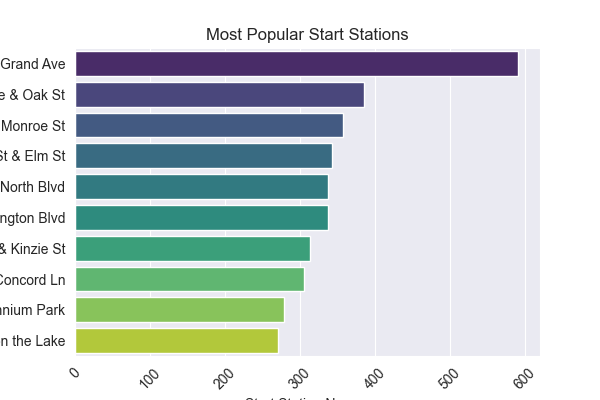
\includegraphics[width=0.8\textwidth]{images/count_most_popular_start_stations}
        \caption{Annual Data Trend}
        \label{fig:graph1}
    \end{figure}


    \section*{Main Questions}
    \label{sec:questions}

    The dataset provides anonymized data of each trip.\newline
    As discussed in Hartman's study~\cite{Hartman2021}, it proposes an approach to asking questions in a financial context. His Article proposes a case study focuses on cost-effective target groups, and which would most benefit the business.\newline
    While this is an intriguing aspect of this dataset. This proposal focuses on the logistics of re-stocking stations. Interpreting User bike collections Patterns based on historical trip records. The list below encompasses proposed questions to guide the data exploration to this goal.

    \begin{itemize}
        \item Which stations are the most used for collections?
        \item Which stations are busier during certain periods of the day?
        \item Which destinations are the most popular among users?
        \item Which periods of the day are these stations most visited?
        \item Which stations should be unloaded while restocking high-demand stations during peak hours?
        \item How do we define peak hours on a location basis? That is, users commuting with shared bicycles, do they have a pattern of behaviour?
    \end{itemize}

    Considering the questions above. The project could extend in scope, covering the pricing model as discussed in Hartman's blog post~\cite{Hartman2021}. However, due to time constraints this project only on the above. On a later section~\ref{sec:future} there's a list of financially related questions.

    \section*{Dataset description}
    \label{sec:dataset}

    The dataset provides historic data~\cite{DataIndex}. Presenting detailed trip information from the Divvy bike-sharing application.\newline
    It Captures the dynamics of bike usage over time and stations. It offers insights into the user's travel patterns.\newline

    This proposal focuses on \textbf{start\_station} and \textbf{end\_station} IDs. Inferencing which stations are in most need of re-stocking. Sourcing bicycles based on the most popular destination.\newline

    The approach would be incomplete, if the analysis doesn't correlate the trip start and end times. Therefore, it's inevitable to analyse the correlation between trip times and stations.\newline

    The analysis proposed doesn't focus on text processing. Nevertheless, I propose storing text-based features, such as station names or member\_casual. That's to enrich the data visualisation with human friendly labels.\newline
    While this approach is not critical for a successful data model training or Analysis. It provides a better experience when visualising the data.\newline
    A good dataset report is only as good as is accessibility.

    \textbf{Dataset Features:}:
    \begin{itemize}
        \item \textbf{star\_ride\_id}: A unique identifier for each trip, ensuring individual trips can be tracked and analyzed discretely.
        \item \textbf{star\_rideable\_type}: The type of bike used for the trip, which can influence usage patterns and availability needs.
        \item \textbf{star\_started\_at}: The timestamp indicating when a trip started, crucial for understanding demand over time.
        \item \textbf{star\_ended\_at}: The timestamp indicating when a trip ended, allowing for the calculation of trip duration and temporal patterns of bike usage.
        \item \textbf{star\_start\_station\_name}: The name of the station where the trip originated, providing a geographic point for demand analysis.
        \item \textbf{star\_start\_station\_id}: A unique identifier for the origin station, which can be used in conjunction with geographic data for mapping and spatial analysis.
        \item \textbf{star\_end\_station\_name}: The name of the station where the trip concluded, indicating the destination demand in the network.
        \item \textbf{star\_end\_station\_id}: A unique identifier for the destination station, useful for spatial analysis and redistribution strategies.
        \item \textbf{star\_start\_lat \& start\_lng}: The latitude and longitude of the start station, giving precise location data for origin points.
        \item \textbf{star\_end\_lat \& end\_lng}: The latitude and longitude of the end station, giving precise location data for destination points.
        \item \textbf{star\_member\_casual}: A categorization of the user as a member or a casual rider, which can influence riding patterns and frequency of use.
    \end{itemize}

    \section*{Method}
    \label{sec:method}
    \begin{itemize}
        \item \textbf{Data Acquisition:}
        \begin{itemize}
            \item The initial phase involves acquiring data from the source.\newline
            By scraping the endpoint available, using a notebook environment to automate the process of scraping. Then, downloading and unzipping, and storing the data files programmatically.\newline
            For the purposes of this proposal, the data is stored in a conventional file storage system and subsequently loaded as a CSV file.
        \end{itemize}

        \item \textbf{Preliminary Setup:}
        \begin{itemize}
            \item While the initial plan was to use Azure Databricks with Azure Datastore as a source in a Big Data framework. However, resource and time constraints necessitated a pivot. Therefore, the data will reside in a local storage.
            \newline Leveraging Apache Spark, and its robust platform for handling large-scale data processing. This project will take a Big data approach in the described context.
            \newline The Azure Databricks approach discussed is based on learnings from Mohit Batra's course~\cite{Batra2022}.
        \end{itemize}

        \item \textbf{Data Pre-processing:}
        \begin{itemize}
            \item The subsequent step involves the pre-processing and cleaning of the dataset, which includes:
            \begin{itemize}
                \item Standardizing features by converting string data types to numeric where necessary.
                \item Scaling the dataset to normalize features for model training, where applicable.
                \item Addressing null values either by imputation or by dropping subsets of data. It depends on the significance of the feature in question.
                \item Removing irrelevant features that do not contribute to the research questions at hand.
            \end{itemize}
        \end{itemize}
        \item \textbf{Feature Engineering:}
        \begin{itemize}
            \item During the pre-processing. Add enrich the dataset by adding a categorical 'date' feature. Segmenting trip times into periods (e.g., morning, afternoon, night). \newline This early inclusion is strategic. To support a supervised learning approach. Considering computational expense and, by extension, operational expenses. Early in the analysis.
        \end{itemize}
        \item \textbf{Exploratory Data Analysis (EDA):}
        \begin{itemize}
            \item During the EDA phase, the project will assess and visualize the clean data.
            \newline Using involve aggregation, counting, and summarizing key features. Employing various graphical representations such as graphs, tables, and heatmaps to identify strong correlations and patterns.
            \newline That will inform the training and refining the models.
        \end{itemize}

        \item \textbf{Refinement:}
        \begin{itemize}
            \item This step builds upon the pre-processing phase by refining features and potentially removing ineffective features based on insights gained from the EDA.
            \newline The objective is to distil the dataset down to the most impactful features that align with the research questions.
        \end{itemize}
        \item \textbf{Model Training and Validation:}
        \begin{itemize}
            \item Two predictive model approaches are proposed and will be evaluated. This can change as the project evolves.
            \begin{itemize}
                \item  A \textbf{classification or clustering model} to identify patterns and groupings within the data.
                \item A \textbf{time series forecasting or regression analysis model} to predict future trends based on historical data.
            \end{itemize}
            The project will explore both approaches. Comparing performance and best fit to the context of this Analysis.

        \end{itemize}
        \item \textbf{Performance Review:}
        \begin{itemize}
            \item Review the performance of each predictive model. Through using a set of metrics appropriate to each model type.
            \newline This could include accuracy, precision, recall, and F1 score for classification models, or mean absolute error (MAE), mean squared error (MSE), and R-squared for regression models.
        \end{itemize}
    \end{itemize}

    \section*{Future Improvements considered}
    \label{sec:future}
    This section briefly discusses ideas for unexplored analysis this project won't cover due to time constraints. However, this student is compelled to mention, as these are valuable venues for further exploration.

    \textbf{Geographical coordinates Analysis for Optimal Bike Redistribution:} \newline
    Future iterations of this project, could lead to a significant enhancement in re-stocking.\newline
    Adding analytical techniques to process and correlate the latitude and longitude of each station. Latitude and longitude features are described on the section~\ref{sec:dataset}\newline
    This more sophisticated approach. Calculates distances between stations, optimizing bike distribution logistics.\newline
    Identifying the nearest overstocked stations to those that are understocked. This approach minimizes transfer times and costs. Resulting in a more efficient company resource allocation when redistributing bikes.\newline
    A further consideration is integration with live feeds. That is, live processing city traffic feeds for live updates. Aggregating the resulting model from geographic coordinates with live feeds. The App could trace the route to its employees.

    \textbf{Financial Context Analysis Expansion:}

    As discussed earlier in the section\ref{sec:dataset}, an alternative venue for exploration is the member usage patterns and their contribution to the overall financial health of the service.\newline
    \newline Key questions that we won't have time to explore in this project.

    \textbf{Here's a brief set of questions considered:}
    \begin{itemize}
        \item Is there a member type that is “best for business”?
        \item The case study describes the pricing model?
        \item Is targeting on casual members, who pay per ride, a better business case?
    \end{itemize}
    \textbf{Suggested venues for analyses are:}
    \begin{itemize}
        \item \textbf{Member Value Analysis:} Assess which member type, \'member\' or \'casual\', generates more value for the business in the long term. This will consider not only direct revenue, but also the operational expenses associated with each user type.
        \item \textbf{Pricing Model Evaluation:} Review the existing pricing model described in the case study. Involves analysing the financial effectiveness of the pricing strategy and identifying opportunities for enhancement to increase profitability without sacrificing user satisfaction.
        \item \textbf{Business Case for Casual Members:} Consider the strategy of targeting casual members who pay per ride. Involves comparing the long-term value of a casual member versus a subscription-based member, considering factors such as ride frequency, duration, and seasonal usage patterns.
    \end{itemize}
    Testing citing from references.bib\cite{DataAnalytics2023}.

    \begin{thebibliography}{9}
        \bibitem{Hartman2021} K. Hartman. \href{https://artscience.blog/home/divvy-dataviz-case-study}{Divvy case study}\/  2021.
        \bibitem{DivvyData} DivvyData bike ride-sharing data \href{https://divvybikes.com/system-data}{Divvy bikes system data}\/
        \bibitem{DataIndex} Index file for historic data \href{https://divvy-tripdata.s3.amazonaws.com/index.html}{Compressed csv files}\/
        \bibitem{Batra2022} M. Batra. \href{https://app.pluralsight.com/library/courses/building-etl-pipeline-microsoft-azure-databricks/table-of-contents}{Building Your First ETL Pipeline Using Azure Databricks}\/ 2022.
    \end{thebibliography}
    \printbibliography

\end{document}
